
%%%% OK

Our solution targets the Android Operating System.
We choose Android because it is the most popular and open-source platform for mobile that is currently available.
Android provides an implementation of the Wi-Fi Direct technology that we use to disseminate data between users.

\subsection{Wi-Fi Direct}

As exposed in Figure~\ref{WiFiVsWiFiDi}, where (a) the Wi-Fi working technology and (b) the Wi-Fi Direct working technology, this last allows to connect two devices together without the requirement of an Access Point.
The Wi-Fi Direct uses peer-to-peer connection types--devices communicate directly together.
We choose the Wi-Fi Direct technology for our proximity dissemination because it covers a wider area than other proximity technologies like the Bluetooth (e.g., Wi-Fi Direct range is more than 600 feet contrary to Bluetooth that is at least 200 feet).
Furthermore, the Wi-Fi Direct technology offers speeds of up to 250 Mbps while Bluetooth is around 25 Mbps.

\begin{figure*}[h]
	\centering
	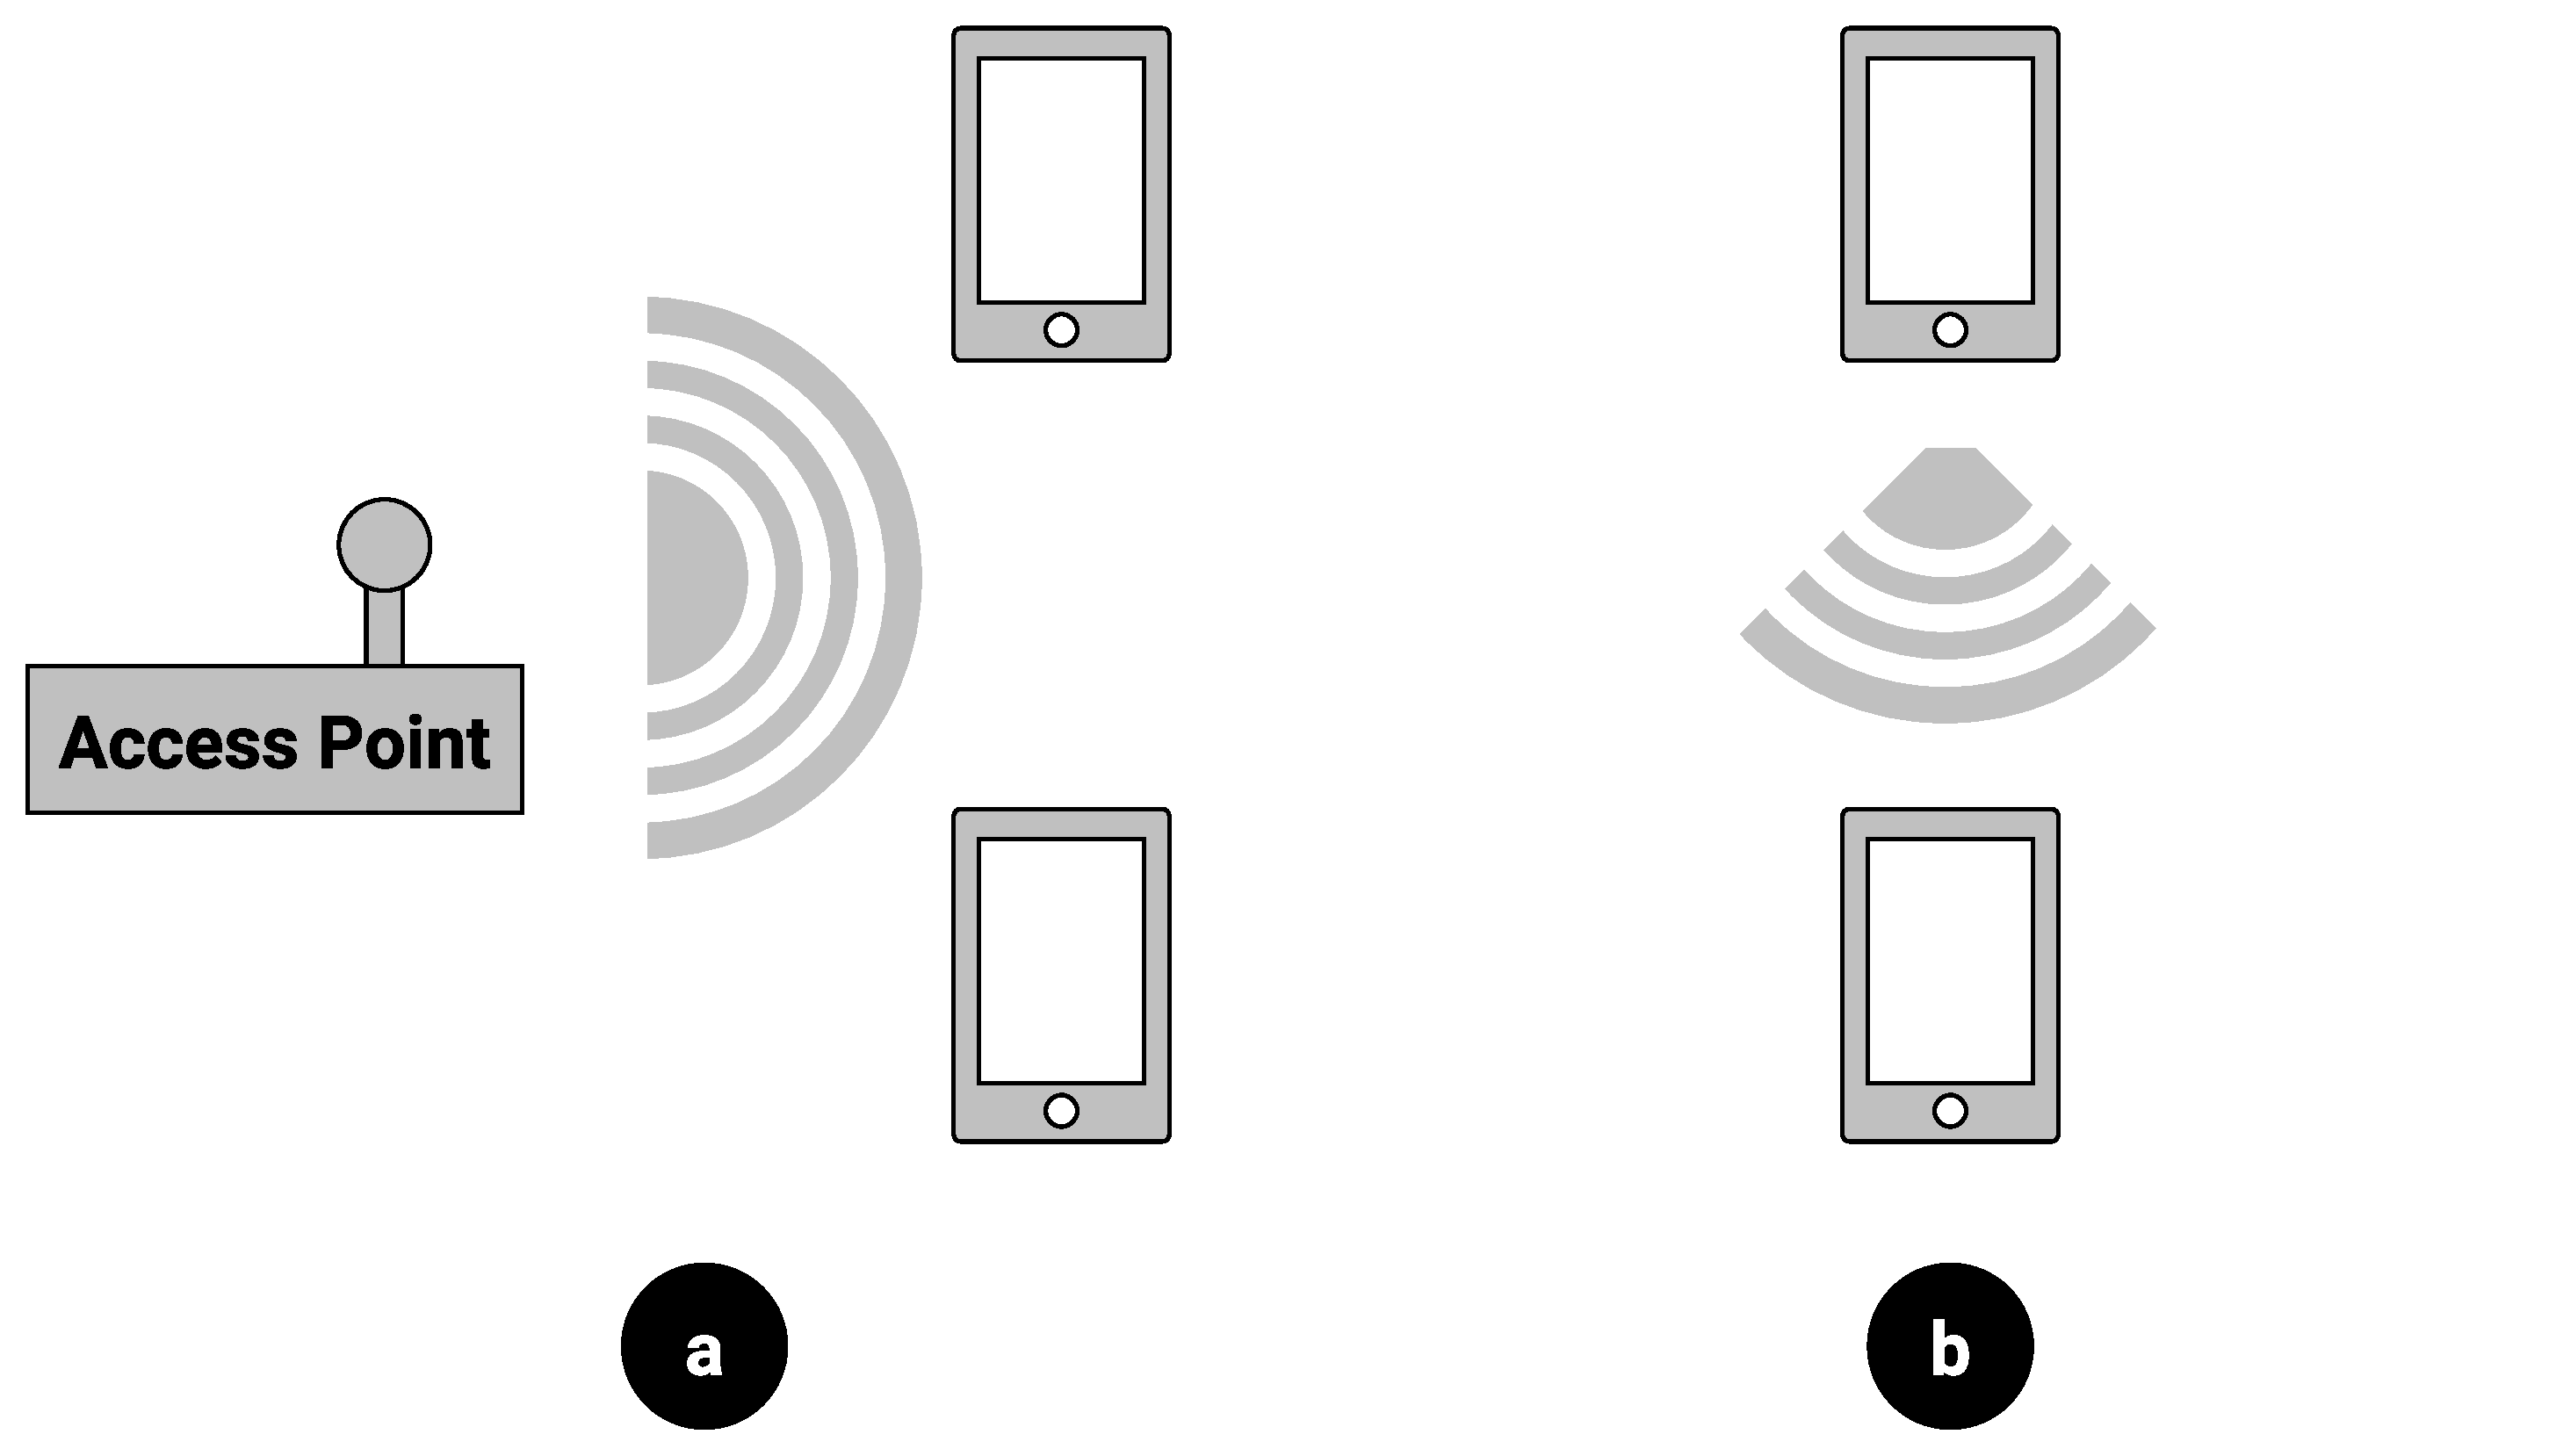
\includegraphics[width=0.7\textwidth]{figures/wifivswifidirect}
	\caption{\label{WiFiVsWiFiDi}Wi-Fi and Wi-Fi Direct network architectures}
\end{figure*}

Before establishing a connection, a device must discover its environment to know if another device is available.
During the discovery process, a device sends regularly a signal that informs about its presence.
The Android Wi-Fi Direct implementation provides the Domain Name System Service Discovery (DNS-SD) protocol that permit to discover other device services that are within range.
This DNS-SD broadcast a set of key/value information that can be read by other devices.
For instance, a broadcast can contain information about the port that will be used to exchange data, the name of the service that is provided, etc.
Devices that are in discovery mode can then filter devices and choose devices that correspond to their connection requirement.
In our implementation, the discovery process is running until the Wi-Fi Direct module is stopped or the Wi-Fi connection is disabled on the device.
\\

After a connection is established between two devices, a private network is created to allow communication through sockets.
The time to establish a connection is about 3 to 5 seconds, but can take up to 2 minutes in the worst cases.
To prevent eventual issues, we set up a timeout to 1 minute per connection.
After this time, device connected or not, the Wi-Fi Direct instance is reset and a new one is instantiated.
The particularity of Wi-Fi Direct communication is that one device on the network is named Group Owner (GO).
The GO is unique for a specific connection and it is the only one that knows all other devices in the private network.
The other connected devices are named Client.
The clients cannot communicate directly with other devices connected to the private network.
They can only communicate with the GO.
\\

This drawback in communication is not embarrassing in our case because we consider that a device can be connected and communicate with only one other device at a time.
In our case, we consider that a device is connected to a single device at a time.
A connection is only made between two devices, no more.
Our implementation does not request for a connection with a device that is already connected with another.
In our implementation, when a connection is successfully processed, each device sends his shared data and add the device to an ephemeral history.
A device is kept in the history an hour to prevent multiple sending of the same data to the same data.
\\

The Wi-Fi Direct implementation requires a user interaction the first time where two devices try to connect each others.
This user's acknowledgement can be seen as a drawback in an opportunistic network because it cuts the flow of hidden interactions between each device, but this interaction requested only the first time a connection is made between two devices.
If the user accepts the connection request, the following connection with the same device will be automatic and do not ask again for user interaction until the next system reboot or Wi-Fi Direct cleaning groups.
A cleaning function that automatically removes the Wi-Fi Direct groups each time the Wi-Fi Direct is started.
We think that the user acknowledgment is important because it enhances the privacy awareness of the user by informing him that his data will be exchanged with another device.
\\

For more details about this technology, a good study made by Conti et al.~\cite{DBLP:conf/wd/ContiDMP13} present specificity of Wi-Fi Direct connections.

\subsection{Peer Sampling Service}

We provide our dissemination solution as a library that can be used in applications that required a data dissemination layer before sending data to a server.
\\

The architecture of the library is exposed in Figure~\ref{Fougere}.

\begin{figure*}[h]
	\centering
	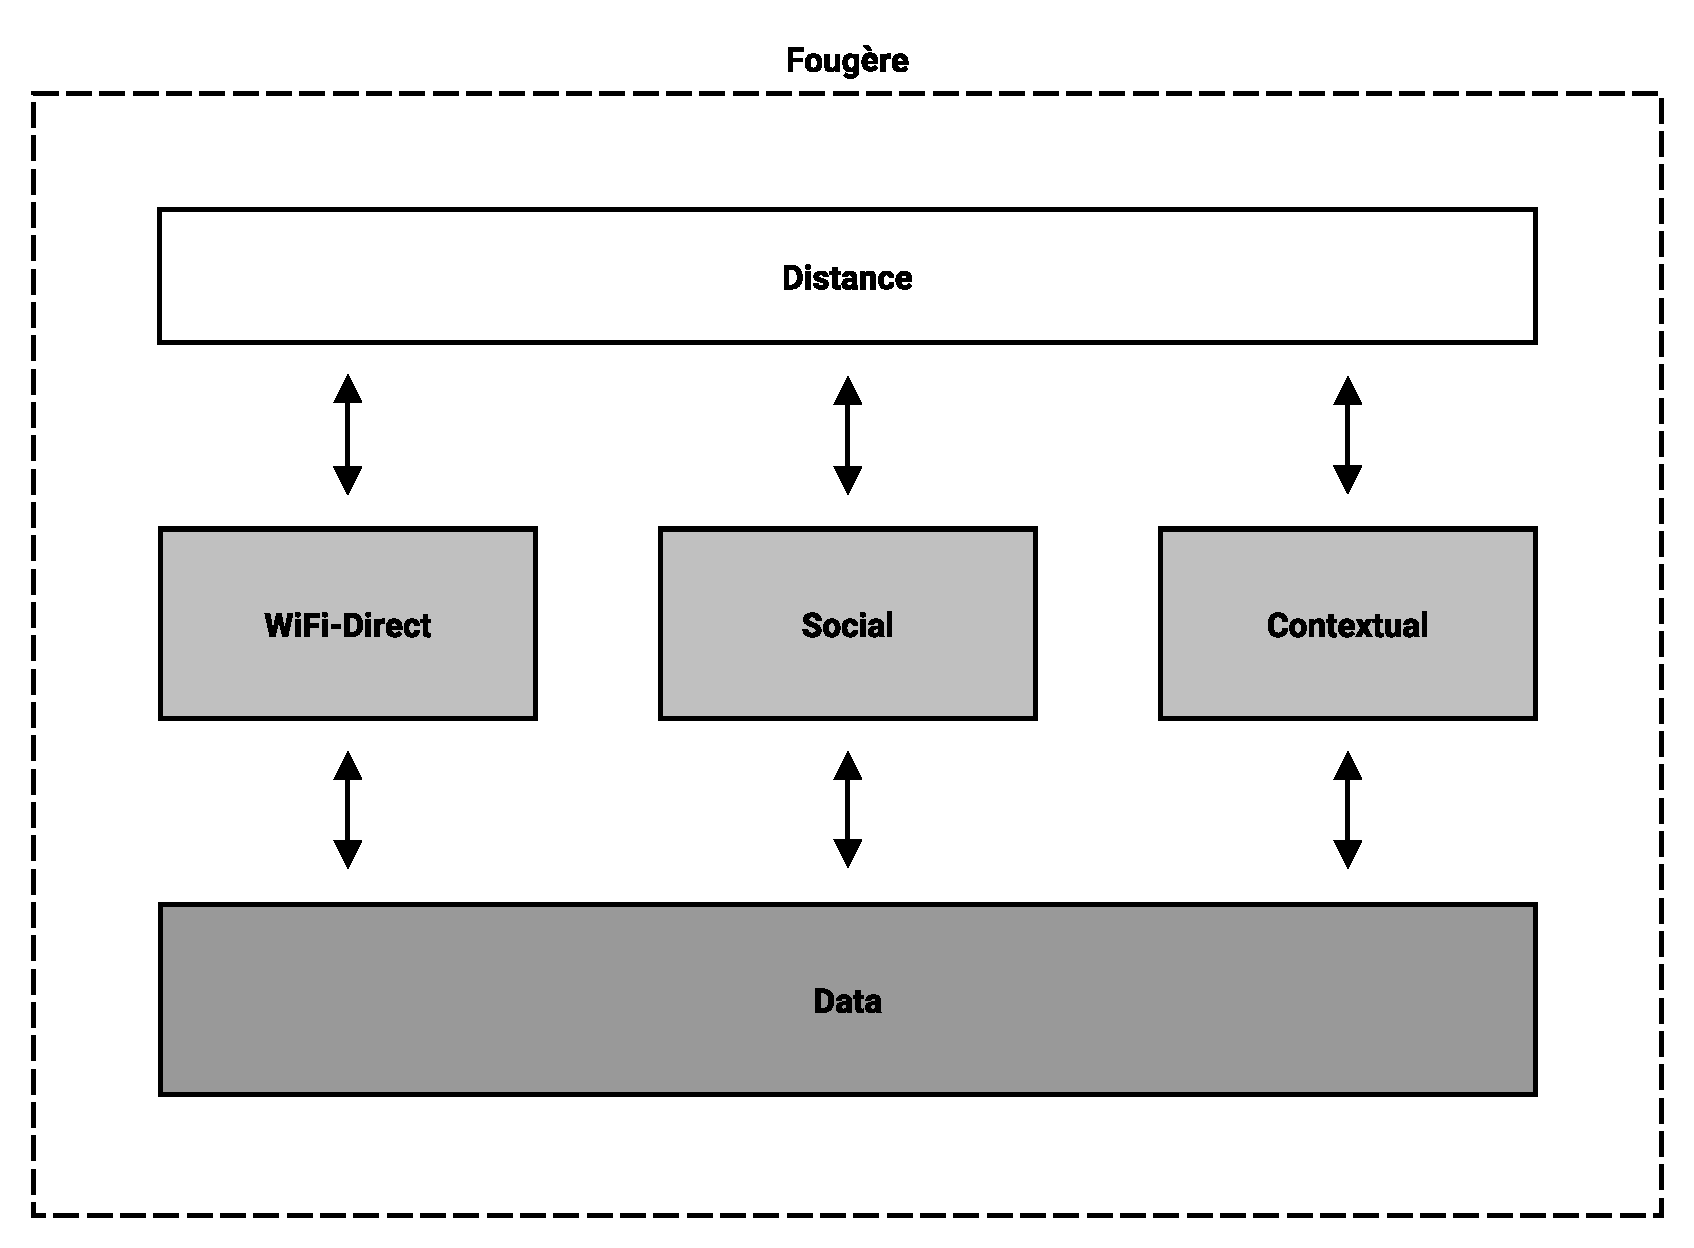
\includegraphics[width=0.7\textwidth]{figures/fougere}
	\caption{\label{Fougere} Foug\`ere architecture}
\end{figure*}

The library includes a database that groups all data that will be disseminated, 3 default modules that are relative to our proposal: \texttt{Wi-Fi Direct} (Physical), \texttt{Social} and \texttt{Contextual} and a \texttt{Distance} class that take choices during the dissemination process.
\\

Foug\`ere has a database that contains all data to disseminate.
This is the application implementing Foug\`ere that fill the database by passing it to the Foug\`ere instance.
A data cannot be in multiple module at a time.
\\

The Distance class is linked with each module.
This is the class that is in charge to determine if the data will be sent to the user.
When a module is able to disseminate data, it requests to the Distance class the ability to disseminate.
According to the status of the process, the module sends it to the Distance which update the user distance value.
\\

Each module needs to be able to receive data because in Foug\`ere, the global data are dispatched at a specific time (e.g., each day at midnight) through the enabled modules.
When the dispatch process is started, all data that are in each module are recovered and regrouped in the global database to be re-dispatched.
By this way, we reshuffle the data and allow to disseminate with another method.
For instance, a data can be sent the first time with the Wi-Fi Direct layer and a second time with the Social one.
\\

The Figure~\ref{WiFiDiServInt} illustrates the process of the Physical type dissemination using the Wi-Fi Direct technology.

\begin{figure*}[h]
	\centering
	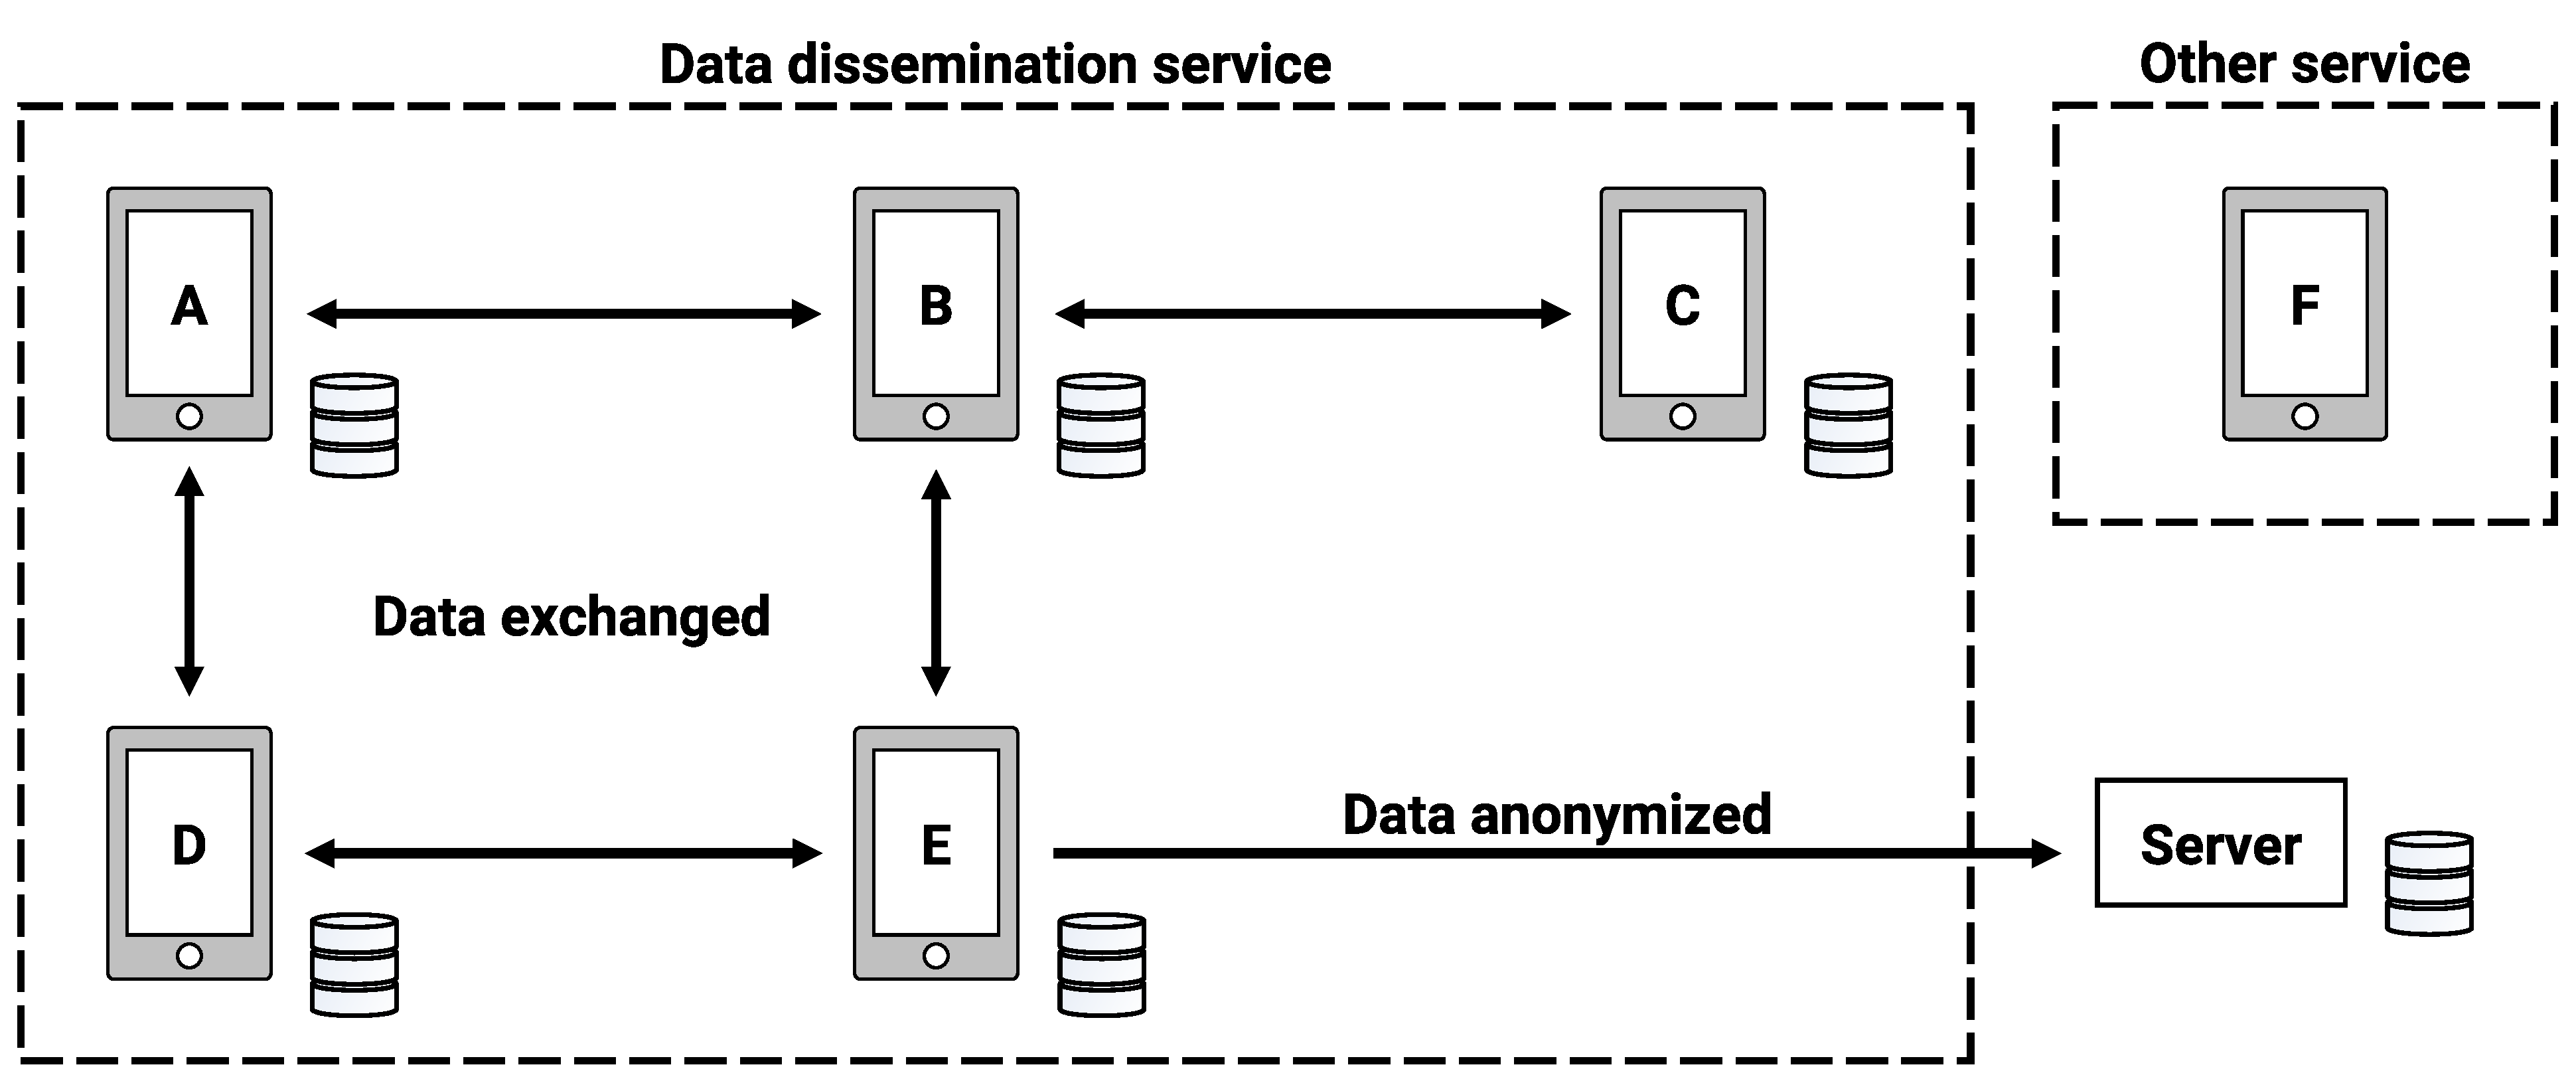
\includegraphics[width=\textwidth]{figures/wifidirect}
	\caption{\label{WiFiDiServInt} Wi-Fi Direct service interactions}
\end{figure*}

As explained above, the Wi-Fi Direct provides a service discovery that allows to provide information during the discovery. 
In this example, the devices A, B, C, D and E provide the data dissemination service where F provides another one.
This indicates that F does not participate in the dissemination and no request will be sent to it by the others.
Where devices are close enough, they can communicate and exchange data.
The data are exchanged and pass through multiple devices.
When the requirements of a data are all reached, the device sends this data to the end-server 

%%%% END OK